\section{Characterizing the Effects of Modelling Uncertainities and Assumptions}
The modelling uncertainities due to the uncertainities in the input definition
and the parameter estimates affect the tracking performance of the controller.
The primary sources of the uncertainities are as follows:
\begin{enumerate}
    \item Uncertainities due to the input definition.
    \begin{enumerate}
        \item Uncertainities caused by neglecting the linear term in the input based on
        the assumptions $b_m = 0 \implies V_{in} b_m u_\omega = 0$.
        \item Effects of non-zero and slowly varying $\delta v$.
    \end{enumerate}

    \item Uncertainities in the model parameter estimates.
\end{enumerate}

The effects of the uncertainities are determined by the relative error in the
prediction from the nominal model and the model with only that particular uncertainity.

\subsection{Effects of non-zero $b_m$}
From the simulink model the uncertainity in $b_m$ does'nt effect the prediction
error significantly. A $3 \sigma$ variation in $b_m$ produced less than $1\%$
relative error in the prediction. Thus, $b_m$ can be completely neglected out of
the non-linear model without significant prediction errors.

\begin{figure}[H]
\begin{minipage}{0.49\textwidth}
    \begin{figure}[H]
        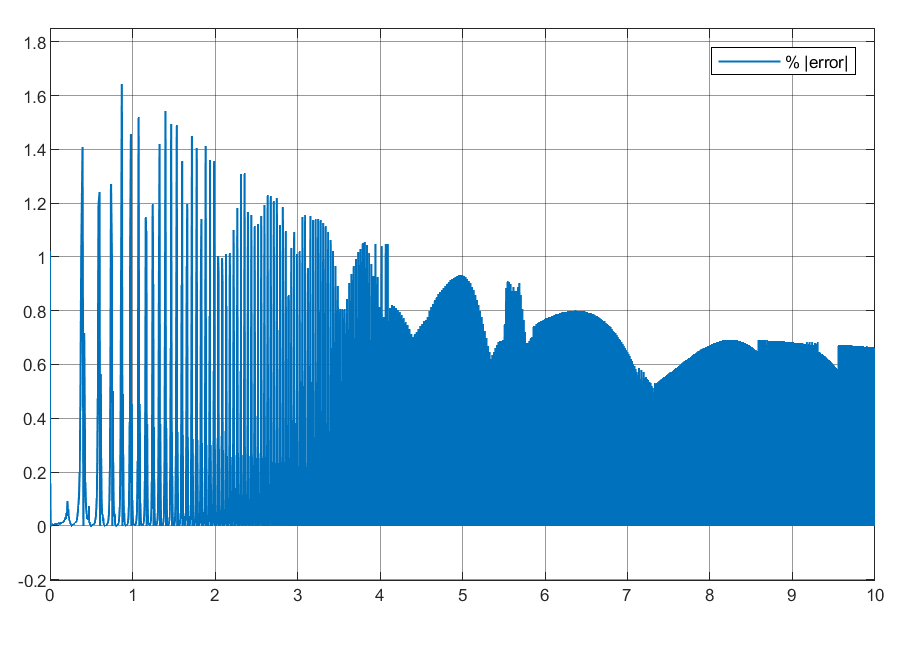
\includegraphics[width = \textwidth]{figs/par_var/3_sig_bm.eps}
        \caption{$\%$ error for $3 \sigma$ variation in $b_m$}
    \end{figure}
\end{minipage}
\begin{minipage}{0.49\textwidth}
    \begin{figure}[H]
        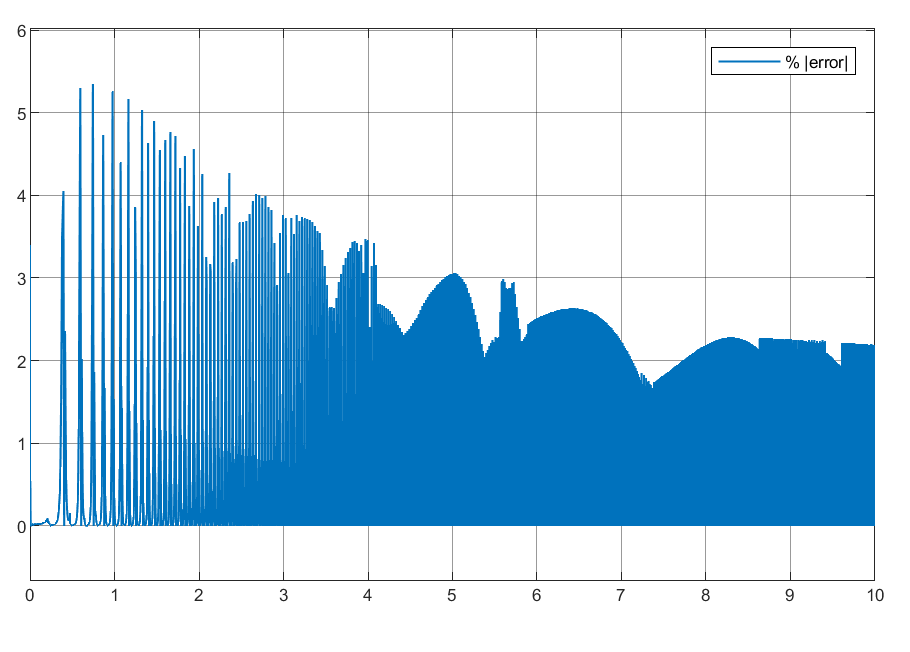
\includegraphics[width = \textwidth]{figs/par_var/10_sig_bm.eps}
        \caption{$\%$ error for $10 \sigma$ variation in $b_m$}
    \end{figure}
\end{minipage}
\end{figure}

\subsection{Effects of non-zero $\delta v$}
$\delta v$ significantly effects the prediction error as it is effectivly
changes the input-gain and also introduces un-compensated friction into the
system.
\begin{figure}[H]
\begin{minipage}{0.49\textwidth}
    \begin{figure}[H]
        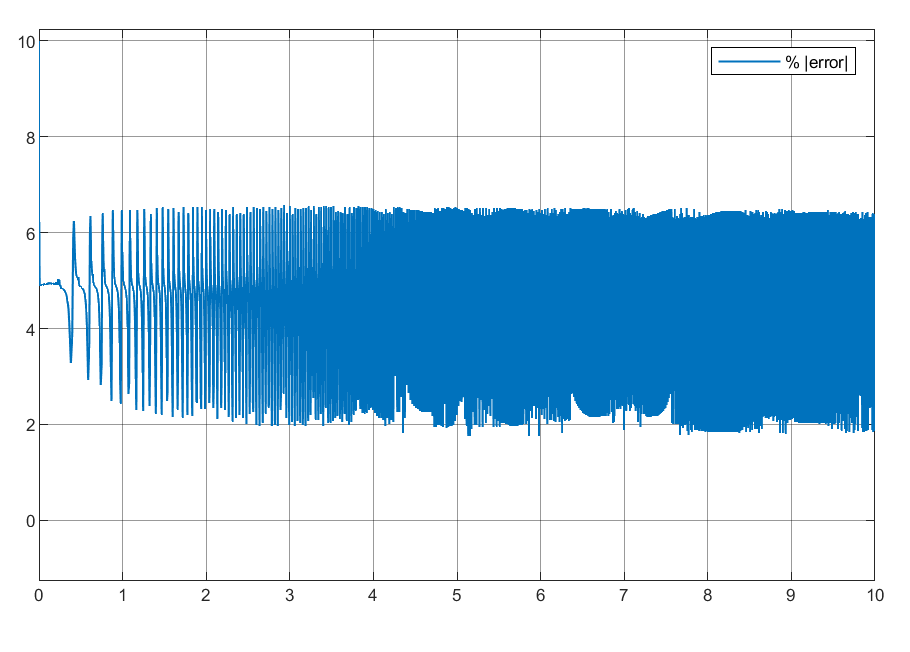
\includegraphics[width = \textwidth]{figs/par_var/1_del_v.eps}
        \caption{$\%$ error $\delta v = 0.1$}
    \end{figure}
\end{minipage}
\begin{minipage}{0.49\textwidth}
    \begin{figure}[H]
        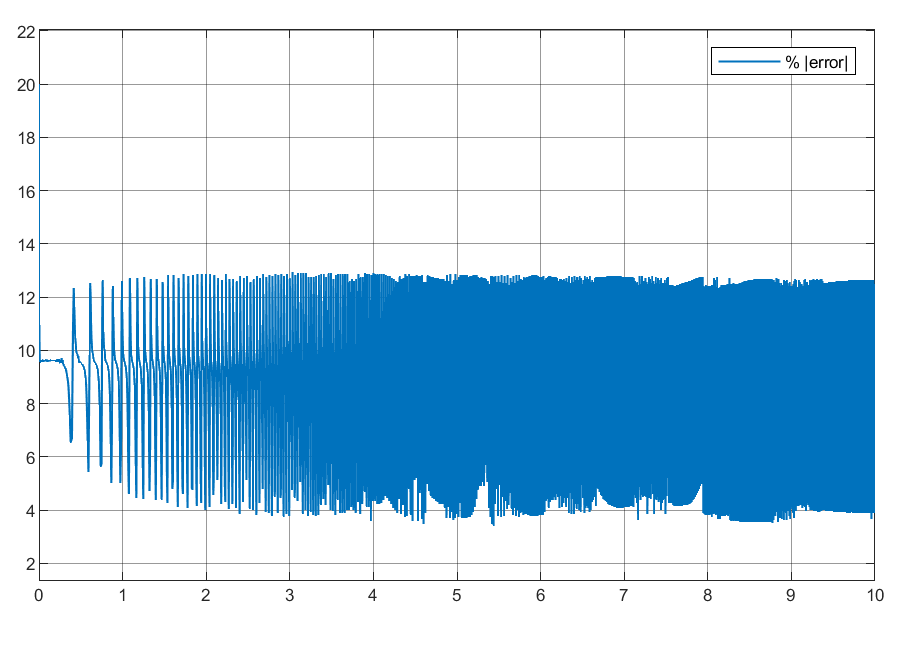
\includegraphics[width = \textwidth]{figs/par_var/2_del_v.eps}
        \caption{$\%$ error for $\delta v = 0.2$}
    \end{figure}
\end{minipage}
\end{figure}


\subsection{Effects of model-parameter estimation errors}
The parameter $J, C_D$ effect the prediction errors to the same order of
magnitude to their estimation errors. The figures bellow show the effect of
$10\%$ estimation errors in their parameters.

\begin{figure}[H]
\begin{minipage}{0.49\textwidth}
    \begin{figure}[H]
        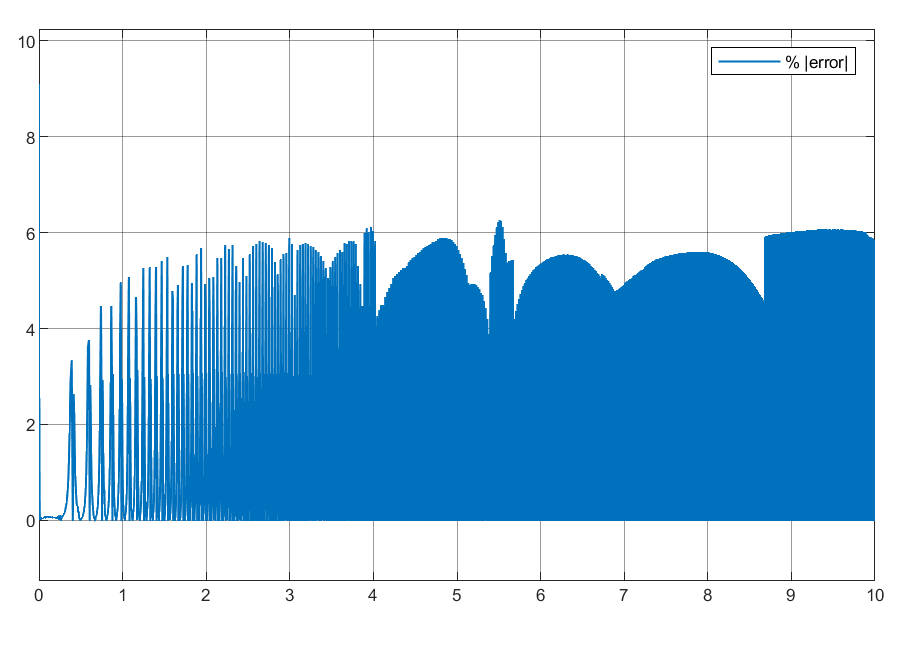
\includegraphics[width = \textwidth]{figs/par_var/j.eps}
        \caption{$\%$ error for $10\%$ error in J}
    \end{figure}
\end{minipage}
\begin{minipage}{0.49\textwidth}
    \begin{figure}[H]
        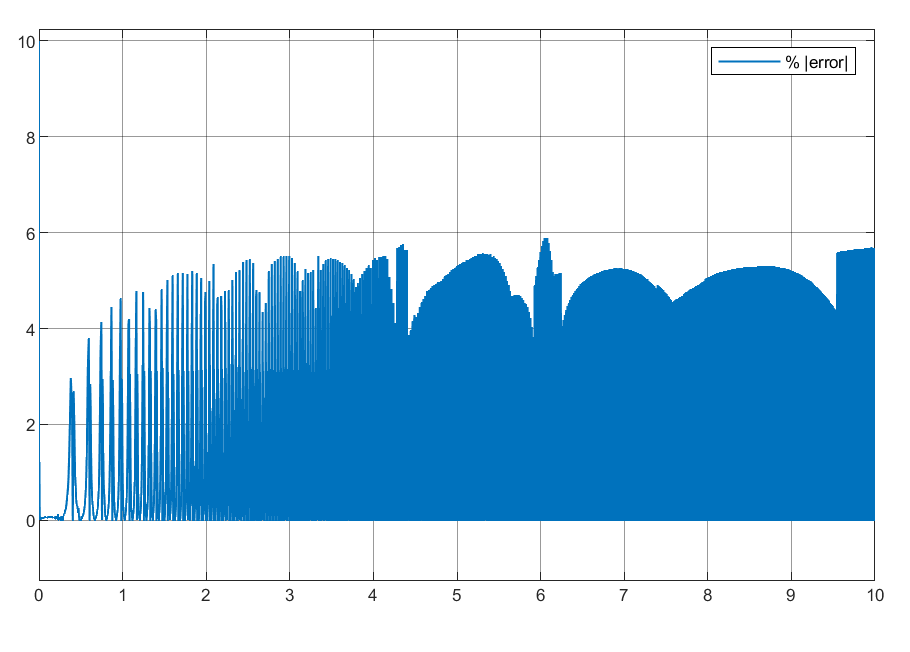
\includegraphics[width = \textwidth]{figs/par_var/c_d.eps}
        \caption{$\%$ error for $10\%$ error in $C_D$}
    \end{figure}
\end{minipage}
\end{figure}

The effect of $M_f$ is indirectly effects $\delta v$. These errors have to be
lumped together for estimation.
    \begin{figure}[H]
        \centering
        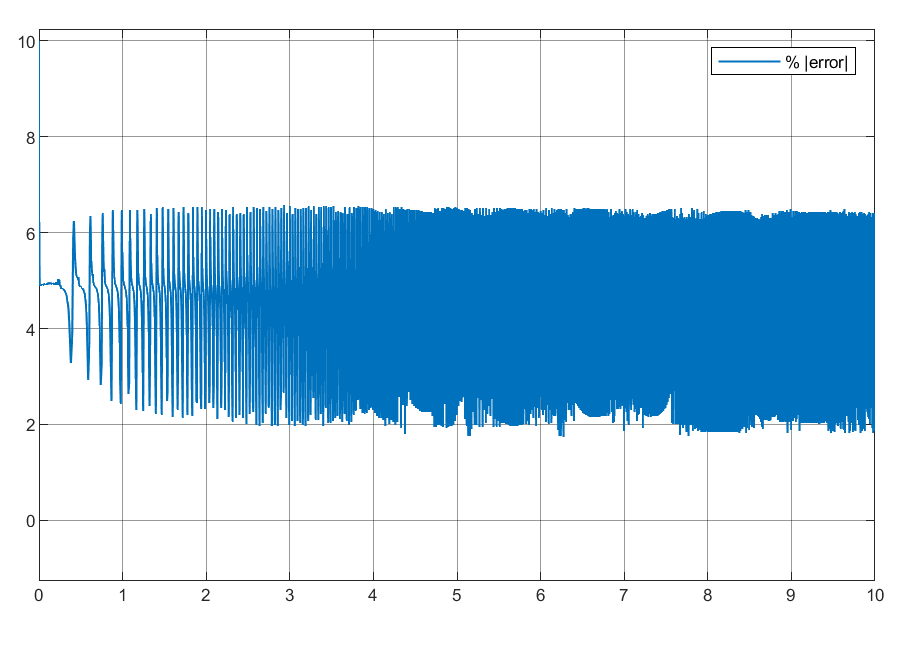
\includegraphics[width = 0.49\textwidth]{figs/par_var/m_f.eps}
        \caption{$\%$ error for $10\%$ error in $M_f$ with $\delta v=0.1$}
    \end{figure}


\subsection{Conclusion}
Thus from above analysis, we conclude following:

\begin{enumerate}
\item The model parameters that significantly effect the tracking performance
are (in the order of their infulunce): $1) \delta v, \, 2) M_f, \, 3)J, \, 4) C_D$
\item The linear damping factor of the motor $b_m$ doesn't significantly effect
the tracking performance of the system with-in it's estimation error. Hence, it can be removed from model simplifiying the model structure and the number of
model parameters to be estimated. Further, this analysis justifies the
assummption used to arrive at the control form \ref{eqn::control_form}. Thus, eqn. (\ref{eqn::control_form}) becomes:
\end{enumerate}

\begin{equation}\label{eqn::no_bm_ctrl_form}
    J \dot \omega + C_D \omega^2 + M_f \delta v = V_{in}^2 (1 + \delta v) C_D u_\omega^2
\end{equation}
